% Based on Template from IIS, ETHz
%%%%%%%%%%%%%%%%%%%%%%%%%%%%%%%%%%%%%%%%%%%%%%%%%%%%%%%%%%%%%%%%%%%%%%%
%%%%%%%%%%%%%%%%%%%%%%%%%%%%%%%%%%%%%%%%%%%%%%%%%%%%%%%%%%%%%%%%%%%%%%%
%%%%%                                                                 %
%%%%%     <file_name>.tex                                             %
%%%%%                                                                 %
%%%%% Author:      Sebastian Thomas                                   %
%%%%% Created:     17.02.2026                                         %
%%%%% Description: <description>                                      %
%%%%%                                                                 %
%%%%%%%%%%%%%%%%%%%%%%%%%%%%%%%%%%%%%%%%%%%%%%%%%%%%%%%%%%%%%%%%%%%%%%%
%%%%%%%%%%%%%%%%%%%%%%%%%%%%%%%%%%%%%%%%%%%%%%%%%%%%%%%%%%%%%%%%%%%%%%%

%%%%%%%%%%%%%%%%%%%%%%%%%%%%%%%%%%%%%%%%%%%%%%%%%%%%%%%%%%%%%%%%%%%%%%%
%%%%%                                                                 %
%%%%%     Document Class                                              %
%%%%%                                                                 %
%%%%%%%%%%%%%%%%%%%%%%%%%%%%%%%%%%%%%%%%%%%%%%%%%%%%%%%%%%%%%%%%%%%%%%%
\documentclass[%
 oneside,      % Use the same margins for odd and even pages (cannot
               % be used with the 'twoside' option). 
% twoside,      % Use different margins for odd and even pages (cannot
               % be used with the 'oneside' option).
 openany,      % Open chapters on odd and even pages.
 halfparskip,  % Create small spaces for new paragraphs but no indents.
]{scrbook}

%%%%%%%%%%%%%%%%%%%%%%%%%%%%%%%%%%%%%%%%%%%%%%%%%%%%%%%%%%%%%%%%%%%%%%%
%%%%%                                                                 %
%%%%%     Preamble                                                    %
%%%%%                                                                 %
%%%%%%%%%%%%%%%%%%%%%%%%%%%%%%%%%%%%%%%%%%%%%%%%%%%%%%%%%%%%%%%%%%%%%%%
% Load the preamble from another file.
\input{./preamble/preamble}

%%%%%
%%%%% Load the glossaries.
%%%%%
% Based on Template from IIS, ETHz
%%%%%%%%%%%%%%%%%%%%%%%%%%%%%%%%%%%%%%%%%%%%%%%%%%%%%%%%%%%%%%%%%%%%%%%
%%%%%                                                                 %
%%%%%     Make Glossaries                                             %
%%%%%                                                                 %
%%%%%%%%%%%%%%%%%%%%%%%%%%%%%%%%%%%%%%%%%%%%%%%%%%%%%%%%%%%%%%%%%%%%%%%

% Required to generate the index for the glossaries.
\makeglossaries

%%%%%%%%%%%%%%%%%%%%%%%%%%%%%%%%%%%%%%%%%%%%%%%%%%%%%%%%%%%%%%%%%%%%%%
%%%%%                                                                %
%%%%%     Definitions of all glossary entries which will appear in   %
%%%%%     the default (main) glossary.                               %
%%%%%                                                                %
%%%%%%%%%%%%%%%%%%%%%%%%%%%%%%%%%%%%%%%%%%%%%%%%%%%%%%%%%%%%%%%%%%%%%%

\newglossaryentry{tecdiving}{name=Technical Diving,description={
While the exact terminology differs between technical divers and agencies, most classify technical diving as every form of scuba diving that includes a virtual or physical ceiling, like decompression ceiling, cave and wreck diving. 
It also includes planning and executing a dive with multiple distinct gas mixes
}}

\newglossaryentry{deco}{name=Decompression,description={
Decompression in diving nomenclature is the process of releasing bound gas from the tissues through breathing a gas that has a lower \gls{pp} of that gas than currently present in some tissue.
In a wider sense, it also includes the specific stop schedule that divers adhere to while ascending
}}

% Add all glossary entries to the glossary, even if they have not been
% referenced.
\glsaddall[types={main}]


%%%%%%%%%%%%%%%%%%%%%%%%%%%%%%%%%%%%%%%%%%%%%%%%%%%%%%%%%%%%%%%%%%%%%%
%%%%%                                                                %
%%%%%     Definitions of all acronyms which will appear in the list  %
%%%%%     of acronyms.                                               %
%%%%%                                                                %
%%%%%%%%%%%%%%%%%%%%%%%%%%%%%%%%%%%%%%%%%%%%%%%%%%%%%%%%%%%%%%%%%%%%%%

\newacronym{aimd}{AIMD}{Additive Increase, Multiplicative Decrease}
\newacronym{bga}{BGA}{Ball Grid Array}
\newacronym{dfn}{DFN}{Dual Flat No-Lead}
\newacronym{qfn}{QFN}{Quad Flat No-Lead}
\newacronym{lqfp}{LQFP}{Low Profile Quad Flat Package}
\newacronym{x2son}{X2SON}{Extra Small Outline No-Lead}
\newacronym{ble}{BLE}{Bluetooth Low-Energy}
\newacronym{cdc}{CDC}{Communication Device Class}
\newacronym{cns}{CNS}{Central Nervous System}
\newacronym{dcs}{DCS}{Decompression Sickness}
\newacronym{dfu}{DFU}{Device Firmware Upgrade}
\newacronym{dfvs}{DFVS}{Dynamic Voltage / Frequency Scaling}
\newacronym{fhe}{FHe}{Fraction of Helium (in a gas mix)}
\newacronym{fn2}{FN2}{Fraction of Nitrogen (in a gas mix)}
\newacronym{fo2}{FO2}{Fraction of Oxygen (in a gas mix)}
\newacronym{gpio}{GPIO}{General Purpose Input Output}
\newacronym{gf99}{GF99}{Gradient Factor 99}
\newacronym{gfhigh}{GF High}{Gradient Factor High}
\newacronym{gflow}{GF Low}{Gradient Factor Low}
\newacronym{hal}{HAL}{Hardware Abstraction Layer}
\newacronym{hpns}{HPNS}{High Pressure Neurological Syndrome}
\newacronym{icd}{ICD}{Isobaric Counterdiffusion}
\newacronym{lsi}{LSI}{Low Speed Internal, real-time oscillator in STM32 MCUs}
\newacronym{lse}{LSE}{Low Speed External, MCU connection for an external oscillator}
\newacronym{mcu}{MCU}{Microcontroller Unit}
\newacronym{msc}{MSC}{Mass Storage Class}
\newacronym{n2}{N\textsubscript{2}}{Nitrogen}
% \newacronym[description={The No Decompression Limit defines the time a diver is allowed at a certain depth without incurring a mandatory decompression ceiling}]{ndl}{NDL}{No decompression limit}
\newacronym{ndl}{NDL}{No decompression limit}
\newacronym{o2tox}{O2 Tox}{Oxygen Toxicity}
\newacronym[description=Oxygen Toxicity Unit (percent of the NOAA-introduced CNS Clock)]{otu}{OTU}{Oxygen Toxicity Unit}
\newacronym{oti}{OTI}{Oxygen Toxicity Index}
\newacronym{o2}{O\textsubscript{2}}{Oxygen}
\newacronym{oc}{OC}{Open Circuit}
\newacronym{cc}{CC}{Closed Circuit}
\newacronym{pcb}{PCB}{Printed Circuit Board}
\newacronym{pp}{PP}{Partial Pressure}
\newacronym{phe}{PHe}{PP of Helium}
\newacronym{pn2}{PN2}{PP of Nitrogen}
\newacronym{po2}{PO2}{PP of oxygen}
\newacronym{rtc}{RTC}{Real-Time Clock}
\newacronym{rtic}{RTIC}{Real-Time Interrupt-driven Concurrency}
\newacronym{scuba}{scuba}{Self-contained underwater breathing apparatus}
\newacronym{swd}{SWD}{Serial Wire Debug}
\newacronym{i2c}{I2C}{Inter-Integrated Circuit}
\newacronym{io}{I/O}{Input-Output}
\newacronym{ic}{IC}{Integrated Circuit}
\newacronym{pbl}{PBL}{Center for Project-Based Learning}
\newacronym{spi}{SPI}{Serial Peripheral Interface}
\newacronym{tbm}{TBM}{Time Between Measurements}
\newacronym{tbe}{TBE}{Time Between Executions}
\newacronym{uart}{UART}{Universal Asynchronous Receiver Transmitter}
\newacronym{vpm}{VPM}{Variable Permeability Model}
\newacronym{wob}{WOB}{Work of Breathing}

% Add all acronyms to the list of acronyms even if they have not been
% referenced.
\glsaddall[types={\acronymtype}]


% Define which source files should actually been processed.
%\includeonly{./content/06-design_implementation}


%%%%%%%%%%%%%%%%%%%%%%%%%%%%%%%%%%%%%%%%%%%%%%%%%%%%%%%%%%%%%%%%%%%%%%%
%%%%%                                                                 %
%%%%%     Document Settings                                           %
%%%%%                                                                 %
%%%%%%%%%%%%%%%%%%%%%%%%%%%%%%%%%%%%%%%%%%%%%%%%%%%%%%%%%%%%%%%%%%%%%%%

%%%%% Mandatory title page settings.
\title{Linear-Exponential Algorithm-based Open Source Dive Computer}
\author{Sebastian Thomas}
\email{tsebastian@ethz.ch}
\date{June 2026}
\semester{Spring Semester 2026}
\reporttype{Bachelor Thesis}
\firstsup{Dr. Tommaso Polonelli, tommaso.polonelli@pbl.ee.ethz.ch}
% \secondsup{PD Dr. Michele Magno, michele.magno@pbl.ee.ethz.ch}
\professor{Prof. Dr. Luca Benini, lbenini@iis.ee.ethz.ch}

%%%%% Optional title page settings.
\titlelogo{./figures/titlepage_logo}  % some nice graphics to show what you did in your thesis
\logoheight{7cm}                      % Height of the title page logo.
\titlepagemargin{3cm}                 % Margin on the title page.


%%%%%%%%%%%%%%%%%%%%%%%%%%%%%%%%%%%%%%%%%%%%%%%%%%%%%%%%%%%%%%%%%%%%%%%
%%%%%                                                                 %
%%%%%     Start of Document                                           %
%%%%%                                                                 %
%%%%%%%%%%%%%%%%%%%%%%%%%%%%%%%%%%%%%%%%%%%%%%%%%%%%%%%%%%%%%%%%%%%%%%%
\begin{document}

% Prepare document for minitoc insertions.
\dominitoc

\frontmatter

% Create title.
% Based on Template from IIS, ETHz
%%%%%%%%%%%%%%%%%%%%%%%%%%%%%%%%%%%%%%%%%%%%%%%%%%%%%%%%%%%%%%%%%%%%%%%
%%%%%%%%%%%%%%%%%%%%%%%%%%%%%%%%%%%%%%%%%%%%%%%%%%%%%%%%%%%%%%%%%%%%%%%
%%%%%                                                                 %
%%%%%     <file_name>.tex                                             %
%%%%%                                                                 %
%%%%% Author:      <author>                                           %
%%%%% Created:     <date>                                             %
%%%%% Description: <description>                                      %
%%%%%                                                                 %
%%%%%%%%%%%%%%%%%%%%%%%%%%%%%%%%%%%%%%%%%%%%%%%%%%%%%%%%%%%%%%%%%%%%%%%
%%%%%%%%%%%%%%%%%%%%%%%%%%%%%%%%%%%%%%%%%%%%%%%%%%%%%%%%%%%%%%%%%%%%%%%
\makeatletter
\newgeometry{margin = \@titlepagemargin}
\begin{titlepage}

 % Remove the page number in the footer.
 \thispagestyle{empty}

 \begin{center}
   \vspace{0pt}	
   
\includegraphics[height=12mm]{./figures/eth_logo} \hfill    
\includegraphics[height=12mm]{./figures/pbl_logo}\\
  \vspace{0.1cm}

  \hspace*{0.15cm}\rule{0.985\textwidth}{0.4pt}

  \vspace{0.5cm}

  {\Large\textsc{Department of Information Technology and \\Electrical Engineering}}

  \vspace{0.2cm}

  \show@semester

  \vfill

  \begin{spacing}{2.0}
  {\Huge\textbf{\@title}}
  \end{spacing}

  \vspace{0.2cm}

  \show@reporttype

  \vfill
  
  \ifx\@titlelogo\@empty
   \relax
  \else
   \includegraphics[height = \@logoheight]{\@titlelogo}
  \fi
    
  \vfill

  {\Large \@author}\\
  {\@email}
  
  \vfill
  
  \@date

  \vfill
  
  \begin{tabular}{ll}
   Supervisor: & \show@firstsup \\
                % & \show@secondsup \\
   \rule{0pt}{3ex}Professor: & \show@professor \\
  \end{tabular}

 \end{center}
\end{titlepage}
\restoregeometry
\makeatother

%\maketitle

% Include acknowledgements, abstract, etc...
% Based on Template from IIS, ETHz
%%%%%%%%%%%%%%%%%%%%%%%%%%%%%%%%%%%%%%%%%%%%%%%%%%%%%%%%%%%%%%%%%%%%%%%
%%%%%%%%%%%%%%%%%%%%%%%%%%%%%%%%%%%%%%%%%%%%%%%%%%%%%%%%%%%%%%%%%%%%%%%
%%%%%                                                                 %
%%%%%     <file_name>.tex                                             %
%%%%%                                                                 %
%%%%% Author:      <author>                                           %
%%%%% Created:     <date>                                             %
%%%%% Description: <description>                                      %
%%%%%                                                                 %
%%%%%%%%%%%%%%%%%%%%%%%%%%%%%%%%%%%%%%%%%%%%%%%%%%%%%%%%%%%%%%%%%%%%%%%
%%%%%%%%%%%%%%%%%%%%%%%%%%%%%%%%%%%%%%%%%%%%%%%%%%%%%%%%%%%%%%%%%%%%%%%

\chapter*{Acknowledgements}
\lipsum[1-2]

% Based on Template from IIS, ETHz
%%%%%%%%%%%%%%%%%%%%%%%%%%%%%%%%%%%%%%%%%%%%%%%%%%%%%%%%%%%%%%%%%%%%%%%
%%%%%%%%%%%%%%%%%%%%%%%%%%%%%%%%%%%%%%%%%%%%%%%%%%%%%%%%%%%%%%%%%%%%%%%
%%%%%                                                                 %
%%%%%     <file_name>.tex                                             %
%%%%%                                                                 %
%%%%% Author:      <author>                                           %
%%%%% Created:     <date>                                             %
%%%%% Description: <description>                                      %
%%%%%                                                                 %
%%%%%%%%%%%%%%%%%%%%%%%%%%%%%%%%%%%%%%%%%%%%%%%%%%%%%%%%%%%%%%%%%%%%%%%
%%%%%%%%%%%%%%%%%%%%%%%%%%%%%%%%%%%%%%%%%%%%%%%%%%%%%%%%%%%%%%%%%%%%%%%

\chapter*{Abstract}
% The \textbf{abstract} is the presentation card of your work, it is fundamental to describe your contribution and relevant results in few lines of text. 
% It must fit in one page and should include:
% \begin{itemize}
%     \item Short description of your topic or use case;
%     \item Short description of existing technology, work, product and the scientific research challenges still unsolved;
%     \item Description of you work and your contribution;
%     \item A short summary of the most relevant results of your work and the conclusions you draw from it.
% \end{itemize}

Dive Computers are now standard equipment for scuba diving, continuously tracking inert gas loading, the corresponding decompression obligation, and oxygen exposure.
They also allow for more detailed dive logging by allowing users to view and export the recorded depth over time.
As safety-critical, battery-powered life-support devices, commercial and military dive computers are frequently based on proprietary hardware and algorithms, limiting customization options, transparency, and reproducibility.
Previous work has shown that adaptive or variable-rate scheduling can substantially reduce computational effort and energy consumption in low-power embedded systems.
Among existing decompression models, the Thalmann-inspired linear-exponential approach has been associated with reduced decompression sickness risk on deeper dives but is rarely implemented, especially in publicly available dive computer software.

This work presents an extendable open-source hardware and software basis for the development of dive computers that is feasible to build and extend for non-professional audiences, while remaining compact enough to be worn during a scuba dive.
The diving-related algorithms for tracking inert gas loading, decompression, and oxygen toxicity are implemented in a separate open-source module.
Multiple algorithms are implemented and used for the variable rate scheduling of different tasks in dive mode.
These algorithms show a reduction in executions from $1.17\times$ to $6\times$ for decompression calculations without significant difference in the resulting simulated dive profiles compared to the fixed-rate baseline, while the oxygen toxicity calculation does not benefit from the current implementation of variable rate scheduling.
Flash logging to accurately reconstruct a dive profile has been reduced by a factor of $3.6\times$ to $4.1\times$ compared to the fixed-rate baseline while incurring no measurable accuracy loss on the simulated profiles.
The usage of the Thalmann-inspired linear-exponential algorithm performs as expected, recommending slightly deeper stops on deep profiles without incurring significant computational overhead.

\include{./content/00_3_authorship}

% Insert table of contents, list of figures, and list of tables.
\tableofcontents
\listoffigures
\listoftables

% Print list of acronyms.
\setlength{\glslistdottedwidth}{0.2\linewidth}
\printglossary[type=\acronymtype,style=listdotted,title=List of Acronyms]


%%%%%
%%%%% Start the actual main content part.
%%%%%
\mainmatter

% Include the actual content files.
% Based on Template from IIS, ETHz
%%%%%%%%%%%%%%%%%%%%%%%%%%%%%%%%%%%%%%%%%%%%%%%%%%%%%%%%%%%%%%%%%%%%%%%
%%%%%%%%%%%%%%%%%%%%%%%%%%%%%%%%%%%%%%%%%%%%%%%%%%%%%%%%%%%%%%%%%%%%%%%
%%%%%                                                                 %
%%%%%     <file_name>.tex                                             %
%%%%%                                                                 %
%%%%% Author:      <author>                                           %
%%%%% Created:     <date>                                             %
%%%%% Description: <description>                                      %
%%%%%                                                                 %
%%%%%%%%%%%%%%%%%%%%%%%%%%%%%%%%%%%%%%%%%%%%%%%%%%%%%%%%%%%%%%%%%%%%%%%
%%%%%%%%%%%%%%%%%%%%%%%%%%%%%%%%%%%%%%%%%%%%%%%%%%%%%%%%%%%%%%%%%%%%%%%

\chapter{Introduction}
Give an overview of the problem, and put your work into a bigger
context. Motivate the questions addressed in this work and summarize
your contributions. 

If you want to \emph{highlight} a word or term use \verb|\emph{}|.

If you work with many acronyms we recommend the use of an acronym library. You can define acronyms in the lower part of the glossaries.tex file. When first using the acronym it will be introduced \gls{pbl}, after that the shortform will be displayed \gls{pbl}.

\gls{scuba} diving is a recreational activity that involves breathing one or more compressed gas mixes.
Dive computers in their most basic form consist of a depth sensor, a real-time clock, processing unit, and a display. 
Their primary function is to display dive time and depth, as well as to calculate and display decompression obligation and \gls{otu}s during the dive. 
Furthermore, most computers show statistics about recent dives or allow downloading the dive logs for further analysis and accurate logging when on the surface.

\section{Motivation}
Dive Computers commonly sample depth and update the corresponding display multiple times per second, while log rate (the stored logs for later retrieval) is usually user-defined between 1 and 30 seconds. Recomputation of decompression schedules cannot be as simply observed; thus, it can only assumed that it happens on a scale of at least every few seconds. 

As Prof Dr Simon Mitchell explains, hyperbaric medicine and especially decompression science is 'bucket chemistry', meaning that the extent to which accurate O2 time and decompression tracking is useful is on the order of seconds. However, this does not mean that more frequent sampling is useless for all applications, most divers rely on their dive computers to refresh the depth display in increments of $\SI{10}{\cm}$ with a sub-second delay. 

However, there is no indication that knowledge about typical dive profiles influences these rates, i.e., there is no research in the public domain that investigates the feasibility of a variable refresh rate for all the previously listed components. 

\section{Objective}
what was the objective of your thesis? also add your research questions here

\subsection{Research Questions}
\begin{enumerate}
\item Is it possible to create a fully Open-Source dive computer which can use both exponential and linear-exponential algorithms, based on the user's preference?
\item Can an appropriately-sized \gls{pcb} be designed and still be hand-soldered?
\item Can sufficiently much energy and log space be saved by employing task variable-rate task scheduling / procedure running to offset the incurred overhead by the variable-rate algorithms?
\end{enumerate}

\subsection{Outline}
First, an introduction to measurement-based embedded devices, energy-saving measures in battery-power devices, and basic hyperbaric medicine theory is presented, to the extent that it is relevant to divers and dive computer developers. 
Next, we look at related work to save energy in embedded devices, mainly by running at tasks variable rate. 
Following this, the specific implementation of this project in hardware and software is described. 
Chapter 5 will collect and compare the results received using different sortware.
Finally, the results will be critically discussed and compared with those in the related work.

% Based on Template from IIS, ETHz
%%%%%%%%%%%%%%%%%%%%%%%%%%%%%%%%%%%%%%%%%%%%%%%%%%%%%%%%%%%%%%%%%%%%%%%
%%%%%%%%%%%%%%%%%%%%%%%%%%%%%%%%%%%%%%%%%%%%%%%%%%%%%%%%%%%%%%%%%%%%%%%
%%%%%                                                                 %
%%%%%     <file_name>.tex                                             %
%%%%%                                                                 %
%%%%% Author:      <author>                                           %
%%%%% Created:     <date>                                             %
%%%%% Description: <description>                                      %
%%%%%                                                                 %
%%%%%%%%%%%%%%%%%%%%%%%%%%%%%%%%%%%%%%%%%%%%%%%%%%%%%%%%%%%%%%%%%%%%%%%
%%%%%%%%%%%%%%%%%%%%%%%%%%%%%%%%%%%%%%%%%%%%%%%%%%%%%%%%%%%%%%%%%%%%%%%


\chapter{Background}
\section{Embedded Systems}
\begin{definition}[Embedded System] An embedded system (or embedded device) is an information processing or specialized computing system for a dedicated task embedded into a larger product, typically under constraints such as real-time behavior, limited resources, and low power consumption.
\end{definition}
Most embedded systems are built around a \gls{mcu}, which exist in different package sizes, differ in clock frequency, memory, and flash size, and are produced by multiple manufacturers, the most common families include the STM32 and ESP32. 
Most \gls{mcu}s include high and low speed (\gls{rtc}) clocks, and to increase accuracy, the option of attaching an external crystal or oscillator is provided.

While some embedded systems execute one or more tasks in response to external stimuli, others schedule tasks at regular or quasi-periodic intervals. 
Embedded systems also differ based on which they are integrated: for example, airplanes and automobiles contain dozens or even hundreds of individual devices that interoperate with one another, each controlling and accessing different peripherals, whereas small embedded devices often perform a single task and operate in isolation, controlling all peripherals.

\subsection{Low Power Consumption in Battery-powered devices}
Power Consumption is often a limiting factor for embedded systems, especially when running off a battery, which should provide sufficient runtime for the device's application. 

Firstly, embedded devices are not comparable to general-purpose computer systems in that their hardware and software are fixed before production, increasing usage predictability and allowing for accurate simulations. 
Usually, only a single or small set of fixed tasks have to be run and scheduled, typical specs for an \gls{mcu} include RAM and flash on the order of dozens of kilobytes to a few megabytes, a CPU clock frequency (usually fixed but software-configurable) on the order of single-digit to hundreds of megahertz, and only the minimum required peripherals and components. 
Special compute power like floating point units and crypto hardware acceleration may be included in some units, while others do not incorporate them.

From a hardware standpoint, component selection can significantly impact battery life, and choosing high-quality low-loss components designed for low voltage and current is usually desirable.

The software also influences battery life, mainly through the efficiency of the algorithms implemented, the definition and usage of provided of sleep modes and interrupt/wakeup handling, and the scheduling overhead of tasks. 
The interrupt controller is a central part of each \gls{mcu}, and the number of available interrupts (internal to the processing unit or external, exposed via \gls{gpio}) differs between packages and units.

\subsubsection{Low-power Modes}
ST Microelectronics provides \href{https://wiki.st.com/stm32mcu/wiki/Getting_started_with_PWR}{multiple low-power modes} in their \gls{mcu}s, which differ in their power consumption and wake-up behavior. 

In sleep, low-power run and sleep and STOP modes, SRAM and peripherals (excluding clocks in STOP modes) remain initialized and are lost the Standby and Shutdown modes, the main power regulator is turned off in all STOP1, STOP2, Standby and Shutdown, and the modes have different available wakeup sources. 
When not running any tasks for some amount of time, lower power consumption and higher wakeup latency can be selected by choosing a deeper sleep mode, depending on the project requirements.

\subsection{Variable-rate scheduling}
As noted above, some embedded systems only react to external events and interrupts, while others need to schedule tasks periodically. 
To save in power consumption, it has been shown to decrease power consumption to schedule tasks at varying rates

\section{Diving and Humans in Hyperbaric Environments}
Due to the increase in pressure of $\SI{1}{\bar}$ for every $10$ meters of seawater, the total pressure of the inhaled gas also increases with depth. The gas mixtures used in scuba diving consist of oxygen, nitrogen, optionally helium, and traces of other gasses, which are present only in negligible quantities. Oxygen is the only of these gasses used in the body; the other gasses are referred to as inert. When breathed at a \gls{pp} exceeding the current saturation, the body tissues begin to saturate with that inert gas until they reach environmental pressure and desaturate when the breathed \gls{pp} is less than the tissue's pressure of that gas. This is not an instant process; it takes some time for a tissue to saturate and desaturate to the inhaled \gls{pp}.

While working in mines or on bridges starting in the 1840s, workers started reporting symptoms, some becoming paralyzed, that were later classified as \gls{dcs}, and air embolisms were determined to be the cause. Later, symptoms were significantly reduced by gradually reducing the surrounding pressure instead of immediately ascending to surface pressure \cite{prev-dci-1908}. 
During the second world war, the German, British, and American Armies simultaneously, but secretly, reproduced the observed symptoms using hyperbaric chambers and developed tables for saturation pressure and time and the corresponding required decompression time and pressure/depth schedule \cite{chamber-divers-2024}. 
Whilst these tables are still taught by agencies and used by divers to perform safe dives, requiring only a timer and a depth gauge to track exposure time and maximum depth, dive computers have become mainstream, allowing for multi-level profiles, by knowing not only the maximum depth and total dive time, but exact time spent at each depth, which is used to model tissue pressure, increasing allowed dive time within the \gls{ndl}.

Tissues in the body ongas and offgas different gasses at different rates, tissue-based algorithms model multiple tissues with halftimes of $\SI{5}{\min}$ up to multiple hours (e.g., $\SI{635}{\min}$ or $\SI{720}{\min}$ in Bühlmann-16, respectively) to keep the modeled supersaturation within experimentally developed tissue-dependent limits, while bubble models aim to limit bubble growth \cite{overview-dci-2024}. These algorithms cannot prevent \gls{dcs} from occurring, as exact physiological factors and processes are not fully determined nor can all required parameters be measured while diving, but by adhering to the limits given by tables and computers, incidence is reduced. 

Oxygen is not an inert gas and is thus not ongassed in body tissues. 
However, there are two risks when increasing and decreasing \gls{fo2} of a gas: hypoxia and hyperoxia. 
The first term represents the lack of oxygen, which for humans occurs at a \gls{po2} of around $.16$, and divers are recommended to breathe gas with a \gls{po2} greater than $.18$ to avoid passing out. 
Oxygen also becomes toxic at high \gls{po2} due to its chemical reactivity, and this effect has been experimentally shown to be more exposed when submerged, which is why the upper \gls{po2} limits for diving are $1.6$ during decompression and $1.4$ or less while working. 
The higher \gls{po2} and the longer the exposures, the higher both risks of \gls{cns} and pulmonary oxygen toxicity, and it can lead to serious short- and long-term medical complications, seizures, and death.
Limits for multiple cases have been experimentally developed and published, among others, by the US Navy and NOAA, in tables and the so-called "\gls{cns} clock".

Keeping track of oxygen intake and \gls{pp} is also a primary function of dive computers and will also be presented in this project. 
Although CNS clock limits are more restrictive than the way most technical divers manage risk and new recommendations have recently been published \cite{RevisedO2Tox2025}, these well-established methods have been implemented in most modern dive computers and will serve as a starting point in this project.

Dive computers not only track single-dive exposures; divers are decompressing for hours after a dive is completed, and repetitive dives (i.e. multiple dives within 48 hours) require the tracking of offgassing time even after the dive is complete.
This is why dive computers are almost never completely shut down, as the real-time clock has to run to track inert gas offgassing and \gls{o2} toxicity reduction at surface pressure over time.

Next, we turn our focus to the hardware and software system.
In low power applications, a \gls{mcu} often serves as the computational heart, combining a number of (mostly digital) inputs, outputs, processing power, memory and flash in one chip with low power consumption, often with the possibility of reducing power consumption while running by employing the use of low energy STOP and Standby modes, \gls{dfvs}, disabling GPIO banks, 

To achieve high-reliability and verifiability, real-time operating systems are often used, which are able to provably schedule periodic and aperiodic tasks (sometimes called jobs) according to a deadline, provided that such a scheduling is feasible within the given constraints.


% Based on Template from IIS, ETHz
%%%%%%%%%%%%%%%%%%%%%%%%%%%%%%%%%%%%%%%%%%%%%%%%%%%%%%%%%%%%%%%%%%%%%%%
%%%%%%%%%%%%%%%%%%%%%%%%%%%%%%%%%%%%%%%%%%%%%%%%%%%%%%%%%%%%%%%%%%%%%%%
%%%%%                                                                 %
%%%%%     <file_name>.tex                                             %
%%%%%                                                                 %
%%%%% Author:      <author>                                           %
%%%%% Created:     <date>                                             %
%%%%% Description: <description>                                      %
%%%%%                                                                 %
%%%%%%%%%%%%%%%%%%%%%%%%%%%%%%%%%%%%%%%%%%%%%%%%%%%%%%%%%%%%%%%%%%%%%%%
%%%%%%%%%%%%%%%%%%%%%%%%%%%%%%%%%%%%%%%%%%%%%%%%%%%%%%%%%%%%%%%%%%%%%%%

\chapter{Related Work}
Describe relevant aspects of related work, make sure to have a good covering of your approach/design with others who did similar things. You will need to compare this related work with your results in the Discussion chapter.
% We expect a lot of citations ~\cite{WIKI:Newton} here. 

Make sure to also give the results of the related work relevant to your thesis presented here, including numbers. Often, at the end of this section an overview table makes sense, where you compare related work for different aspects related to your own  thesis.

\section{Diving Algorithms and Dive Computer Hardware Implementation}
There are not many publications related to diving outside hyperbaric medicine, which serve only as a limited reference for the implementation of decompression and oxygen toxicity calculations developed in this project, especially for variable-rate research, as it is relevant for dive computers.
The algorithms have been researched and compared both from a medical and computational perspective, notably the \gls{vpm} algorithm being more computationally complex than Bühlmann's ZHL and similar algorithms \cite{understanding-modern-dive-computers}.

Furthermore, though diving has become a more mainstream hobby over the past 40 years, much research into wearable dive computer technology takes place in a commercial settings, which is not published, so the aim in this case is to provide an extendable Open Source hardware and software platform.

From a medical perspective, Prof. Simon Mitchell confirmed that the recalculation rate of diving algorithms for scuba diving is on the order of seconds, not milliseconds or tenths of milliseconds, calling it "bucket science" \cite{2025-mitchell-personal-comm}.

\section{Low-Power Algorithms and Variable-Rate Research}
For low-power hardware and firmware design, multiple approaches have been evaluated on different platforms, and these influence the development of this project.

In \cite{survey-adaptive-sampling-filtering}, multiple approaches to Adaptive Sampling and Filtering in the context of IOT devices are discussed. 
While not an IOT device, but a wearable, the context of this work resembles the Adaptive Filtering techniques insofar as a boolean decision (transmitting or processing data) is derived from the sampled data, but the algorithms are not filters in the signal processing sense.
The behavior of the system reacts online to sensor samples.

In the following, multiple algorithms are discussed that have been proposed to calculate the dynamic sampling or filtering rate.

Energy-aware approaches take into account battery status and harvesting rate to achieve self-sustaining operation of IOT devices while keeping the sampling rate as high as possible \cite{2023-eth-energy-aware}, using an algorithm  similar to Reno's \gls{aimd}.
The sampling rate is inverse to the one used in this paper, reducing the rate additively and increasing it multiplicatively to avoid frequent sampling when the battery runs out.
The proposed algorithm is lightweight, requiring 527 cycles per iteration, while achieving between $2.06\times$ and $8.68\times$ as many sensor samplings ("localizations") on average.

In \cite{2020-dsra}, adaptive sampling based on changes in the data to sample has been researched, by deriving the sampling rate from the difference between consecutive samples. 
Introduces \gls{tbm} (the name adapted in this work to \gls{tbe}), which is calculated using formula \ref{align:tbm-dsra} as the basis, with $E$ as the so-called exploratory value, the normal sampling rate, $y_i$ and $M_i$ sensor reading and measurement time at time $i$. 
This work produces independent \gls{tbm} values, i.e., the sample rate does not depend on previous executions of the algorithm and can thus be calculated in a stateless fashion.
They note that in some cases, the two current most recent samples do not provide sufficient and relevant data, but rather to use processing before calculating \gls{tbm}. 
The technical results in this paper are not of interest in the context of this work.

\begin{align}\label{align:tbm-dsra}
    TBM = E - \left(S * \left|\frac{y_i - y_{i-1}}{M_i - M_{i - 1}}\right|\right)
\end{align}

In the Adaptive Selection Algorithm for ISP Adaptive Filtering proposed in \cite{QAISAR2019106462}, a window of samples that is passed into the filter is filled until the next run. Absolute limits on the sampling window size and maximum duration are used to avoid missing many samples or only receiving stale data. 
Quantitative analysis yields a reduction of $6.1\times$ to $567\times$ in additions and multiplications compared to other algorithms in test datasets, but these results are combined from the entire processing pipeline and not only the ASA algorithm.

In this work, pressure sampling is performed in regular intervals and variable algorithms use the results from this sampling. 
Therefore, all the papers above provide limited reference and comparison as to the extent to which the adaptive rate processes in this project can benefit the energy consumption.

\chapter{Implementation in Hardware, Firmware and Algorithms}

\section{System Requirements}
The Dive Computer should be able to accurately measure ambient pressure, compute and display depth, decompression, and \gls{o2} toxicity while diving and also on surface breaks, log events to flash, and allow for log download. The display must be large and clear enough to be readable in low-light and low-visibility conditions. The device should be waterproof and resistant to absolute pressures greater than $\SI{4}{\Bar}$.

The battery should last for at least five dives with on average $\SI{90}{\min}$ per dive, for each dive, including the download of the dive log.

To fulfill these requirements, a wireless approach has been chosen, induction is used for wireless battery charging, while \gls{dfu} and dive log download are performed by \gls{ble}.

In order to save power, three distinct modes are implemented, dive mode, bluetooth, and surface mode, where the first measures depth and tracks \gls{deco} and \gls{o2} toxicity on a sub-second scale, while the latter two only measure ambient pressure every few seconds and enable surface communication when necessary.

The screen has been determined to be at least $\SI{1.8}{''}$ large and full-color to be well-visible even in low-light and low-visibility conditions underwater, and to fit the low-power requirements and since most of the display will be black during operation, an OLED screen is appropriate.

\section{Hardware}\label{section:hardware}
\subsection{Component Definition}\label{subsection:definition}
The STM32L476 MCU is used as the computational heart of this project, providing protocol support for \gls{i2c}, \gls{spi}, \gls{swd} and \gls{uart}. It has low power consumption, supports multiple sleep modes, and many software and help resources are available on the internet.

The MS5849-30BA is used as a pressure sensor, it is rated down to a depth of almost $\SI{300}{\m}$ ($\SI{30}{\Bar}$) and provides a base accuracy of a few centimeters, provided optimal conditions. 
To reduce pressure drift, a supply voltage of $\SI{3.3}{\volt}$ has been chosen, although the sensor would be able to run with $\SI{1.8}{\volt}$. 
The total error at extreme temperatures and pressures should be less than $\SI{0.04}{\bar}$, which is approximately $\SI{0.4}{\text{msw}}$. 
It includes an ADC, has direct SPI and I2C pinouts to make it easy to interface with, and development boards compatible with the Click boards\texttrademark\ standard are available. 

The STM32's LSI is not accurate enough for the timekeeping requirements of this project, therefore an external oscillator with a standard frequency of $\SI{32768}{\Hz}$ is used.

To verify power and active dive mode, Bluetooth active and Battery Charging, four LED have been added, a red LED to confirm power on \SI{3.3}{V}, a blue LED that is turned from a GPIO pin on the MCU while in dive mode, an orange LED on the charging IC to show charging status, and a green LED on the $P0\_2$ output of the Bluetooth Transmitter IC.

For debugging purposes, 4 test-points for UART and a 6-pin pad-header for SWD are exposed, both including $\SI{1.8}{\volt}$ and GND header for reference.

To meet the power requirements, an SMD JST PH Connector is provided on the PCB, which is connected to a Li-ion battery with $\SI{3.7}{\volt}$ and a capacity of $\SI{1500}{\milli\ampere{}\hour}$. This also requires the use of dedicated battery protection and charging \gls{ic}s. 
The effective battery output voltage is referred to as $V_{BATT}$ in this thesis and ranges from $\SI{3}{\volt}$ to $\SI{4.2}{\volt}$.
Most components require $\SI{1.8}{\volt}$ (\gls{mcu}, Flash) and $\SI{3.3}{\volt}$ (Pressure Sensor, LEDs, Bluetooth Module), which are generated using a fixed-voltage Dual Step-Down Converter.

A Newhaven Display $\SI{1.8}{''}$ full-color 160x128 OLED display (160128B) and a Microchip RN4871 \gls{ble} module for Bluetooth communication are connected to the \gls{mcu} with \gls{spi} on separate buses. 
The display requires multiple reference voltages, defined in this project (within the constraints given by the datasheet) as $V_{DDIO} = \SI{1.8}{\volt}$, $V_{DD} = \SI{2.5}{\volt}$, and $V_{CC} = \SI{17}{\volt}$. $V_{DDIO}$ is already available on the PCB, $V_{DD}$ and $V_{CC}$ are generated using an LDO from $\SI{3.3}{\volt}$ and a step-up DC-DC PWM converter from $V_{BATT}$, respectively.

\section{PCB Design}\label{section:pcb}
To reduce production cost, a layer count of 4 has been chosen for the PCB, including two ground planes to provide a stable reference to the signals on the remaining two layers. The ground planes are on layers 2 and 4 to reduce the impact of the inductive charging coil, which is placed adjacent to layer 4, instead of the typical layers 2 and 3. All Power is routed using traces and filled zones on layers 1 and 3 of the PCB, the latter are used in dedicated places like the battery connector, DC-DC converters, and power supply for components with higher current draw such as the display $V_{CC}$ and the pressure sensor.

The PCB has dimensions of $\SI{38}{\milli\meter}\times\SI{48}{\milli\meter}$, the 64-pin \gls{mcu} \gls{lqfp} is located in the center, the battery connector, charging, status \gls{ic}s and converters are in the upper left quadrant, display \gls{io} and power converter in the lower left quadrant, while the right side holds, starting in the lower right corner, the Bluetooth module, flash, debug connector, debug LEDs, pressure sensor and UART test pads. 

All resistors and capacitors are of size 0402 (1005), LEDs 0603 (1608), two inductors 1210 (3225) and one inductor 1812 (4532), and most larger components are \gls{lqfp} packages, with the following exceptions. There are three \gls{bga}-mount (battery status and power MOSFET for display and Bluetooth), two \gls{qfn} (pressure sensor and battery charger), one \gls{dfn} (dual step-down converter) and one \gls{x2son} (I2C level shifter) components. Lastly, two Schottky diodes of Metric 0603 size are used. To connect external components, a 34-pin FFC connector for the display and a 3-pin JST PH connector for the battery are present on the board.

All components have been soldered by hand using pneumatic solder paste dispensers, placed with a pair of tweezers, and reflowed using a $\SI{250}{\celsius}$ heating plate. This process is difficult, especially for the display connector and the non-\gls{lqfp} components.

\section{Firmware}\label{section:firmware}
% C Bootloader?
The Firmware has been written in the Rust programming language, using the \lstinline{no-std} environment due to non-availability of a dynamically-allocated objects without a heap. Multiple experimental features like \lstinline{const generics}, \lstinline{const trait implementations} and more \lstinline{const} features are used to achieve the highest performance predictability and avoid runtime overheads. 

In Rust, an important concept is the so-called \href{https://doc.rust-lang.org/beta/embedded-book/static-guarantees/zero-cost-abstractions.html}{Zero Cost Abstraction}, originally a principle defined by Bjarne Stroustrup, creator of the C++ programming language.
Features such as zero-size types (including custom abstractions, like the ones used for pressure units in the algorithm implementations), iterators, and more enable writing very readable code while incurring no performance loss, which is especially important in the embedded environment where every cycle counts to reduce energy.

\subsection{RTOS}
\gls{rtic} has been chosen as a task and concurrency management framework. It is not a full RTOS, as it does not include a kernel or \gls{hal}, relying on external crates, described in the dedicated subsection \ref{section:hal}.

\gls{rtic} uses procedural macros for modules and functions to configure the app and tasks.

\begin{itemize}
    \item \lstinline{rtic::app}: The main \lstinline{mod}
    \item \lstinline{rtic::init}: \lstinline{fn} run at startup to set up peripherals
    \item \lstinline{rtic::idle}: \lstinline{fn} run (while) no other task is running
    \item \lstinline{rtic::task}: \lstinline{fn} to be scheduled as tasks
\end{itemize}

Tasks are scheduled by calling \lstinline{my_task::spawn} for each execution, where \lstinline{my_task} is the name of the task function. There are five tasks in the implementation:

\begin{itemize}
    \item \lstinline{init} to initialize peripherals, and calling the two main tasks \lstinline{task_mode_tick} and \lstinline{task_battery_update}
    \item \lstinline{idle} as an infinite loop waiting for interrupts or other running instructions, which is preempted by RTIC as soon as another task may be run
    \item \lstinline{task_mode_tick} is the main loop that performs functionality based on the current mode
    \item \lstinline{task_battery_update} running at a fixed rate ($\SI{30}{\second}$) to update the current battery, spawning itself again
    \item \lstinline{task_bluetooth_mode} 
\end{itemize}

After waking up from STOP2, registers, RAM and most peripherals keep their state, but it is required to reinitialize the clocks because STOP2 mode might reset the clock tree, PLL, SYSCLK and associated timers and delays. To implement this, the \lstinline{unsafe} \lstinline{Peripherals::steal} functions of the \lstinline{cortex_m} and \lstinline{stm32l4xx_hal::pac} need to be used to access the hardware peripheral registers, this is safe here because only \lstinline{init} used these before, which is exited before \lstinline{task_mode_tick} can be called.

Accessing resources in RTIC is possible via locals and globals, which are passed as context to a task. Locals can only be used by a single task, whereas globals can be used by any task (and represent shared memory). The shared objects are the \lstinline{struct} is \lstinline{latest_measurements}, this is mostly to be able to write and read battery status from both the dedicated battery and the main task, as well as three peripheral access objects to allow reading and writing to the flash from multiple tasks. 

The main task \lstinline{task_mode_tick} multiplexes between two different modes (dive mode and surface), runs one tick of the respective mode, and changes the mode if required.
It is an infinite loop inside an \lstinline{async} function, which \lstinline{await}s the delay between two executions asynchronously, allowing RTIC to schedule another task.

\subsection{\gls{hal}}\label{section:hal}
The standard package to access abstracted peripherals on ARM Cortex-M \gls{mcu}s is the \href{https://github.com/rust-embedded/cortex-m}{\lstinline{cortex-m} (and \lstinline{cortex-m-rt})} crate, which provides wrappers around core peripherals, for example SysTick, registers like MSP and BSRR, and functionality around startup and interrupt handling, including the NVIC (Nested Vector Interrupt Controller).

The \gls{hal} expanding the functionality of the general \lstinline{cortex-m}, which is specific to the \gls{mcu} family, used in this project are maintained and provided by the community project \href{https://github.com/stm32-rs}{\lstinline{stm32-rs}}, specifically the \href{https://github.com/stm32-rs/stm32l4xx-hal}{HAL crate for the STM32L4xx \gls{mcu}s} is used.

\subsection{Low-Power Task Scheduling Algorithms}

\section{Diving Algorithms}\label{section:algorithms}
The algorithms described in this section are implemented in a Rust in a \hyperlink{https://github.com/SebastianThomas/STDC-thalmann}{dedicated repository}, available under the MIT License. The repository is provided for research and educational purposes only. No warranty or guarantee is provided regarding the correctness, reliability, or suitability of the implementation for real-world diving or other safety-critical applications, and the author assumes no liability for any damages, injuries, or losses resulting from its use.

\subsection{Exponential Decompression Algorithm}
The most common decompression algorithms used for recreational and technical diving within the limits of most diving agencies are the Bühlmann-16 family (B, C) and RGBM models. 
The first implemented algorithm is close to the Bühlmann-16C algorithm, an exponential tissue-based algorithm that considers an M-Value (the maximum allowed supersaturation) per tissue, and whenever this value is reached, a decompression stop is added, until the next stop depth can be reached without going beyond the M-Value. 
This experimentally determined M-Value line is often considered too aggressive, so two parameters, \gls{gflow} and \gls{gfhigh}, influence the percentage of M-value the tissues are allowed to reach at the start of decompression (\gls{gflow}) and at the end of decompression, when ascending to the surface (\gls{gfhigh}), between which a linear interpolation of these two points is followed. The parameter \gls{gf99} tracks the minimum distance to the M-Value over all tissues, it is controlled not to exceed the interpolated line in the Bühlmann Algorithm.

\subsection{Linear-Exponential Decompression Algorithm}

\subsubsection{Violations of Henry's Law} 
Usually, gas exchange between tissues is limited by Henry's Law, and follows an exponential relationship.
In \cite{diff-lim-deco-2003}, the authors claim that due to physiological limitations related to the fixed size of the diffusion region in which gas exchange takes place, there may be a limit to the maximum decompression that can occur at a specific depth that does not depend on the \gls{pp}-gradient between neighboring tissues. 
Deeper diving is statistically related to a higher incidence of DCS \cite{dan-understanding-dcs-2022}, therefore, taking precautions such as limiting the amount of decompression (and, with this, also reducing decompression stress) can be beneficial.
This is the theoretical basis for transitioning to another type of function to model decompression in these cases, and only comes into effect on deep technical dives, where the physical exchange limit is smaller than the calculated diffusion allowed by the supersaturation gradient. 
When this point is reached, the modeled change in decompression achieved through an in- or decrease in pressure in the diffusion region only is exactly this change, yielding a linear relationship.

\subsubsection{Iso-\gls{dcs} risk algorithms} 
Bühlmann-16 and RGBM are deterministic \cite{dev-iso-risk-1996}, they consider the safety of a dive profile binary; safe or unsafe, although this is not a realistic model, as these dives still have some remaining risk of DCS based on the physiology of divers that differ between individuals or even the same individual on multiple days. 
These algorithms also fail to take into account the already accumulated and total decompression stress, which can increase the risk of \gls{dcs}, and is often generated by deep dives requiring a long decompression.
The US Navy and similar large organized entities often require a more predictable risk management strategy, and the \gls{dcs} risk should not increase with the parameters of a specific dive. 
Iso-probabilistic \gls{dcs} risk algorithms have been developed to model and execute dives with similar risk at varying depths and bottom times by integrating cumulative decompression stress into a continuous probability function \cite{likelihood-dcs-1984}.

\subsubsection{Thalmann and implemented Linear-Exponential Algorithm}
The linear-exponential decompression algorithm in this project is based primarily on the factors mentioned above. The Thalmann Algorithm \cite{thalmann-tables-software-2010} \cite{thalmann-parameters-1.3-2020}, designed by Capt. Edward D. Thalmann, MD, US Navy, also follows these principles and is used as a reference for the parameters.  

It should though not be assumed that the implemented algorithm is equivalent to the Thalmann algorithm, instead, it builds on the most important ideas and results from the paper and provides a simple, extendable implementation of a linear-exponential decompression algorithm that can easily be exchanged for other algorithms and provides reasonable results for the tested profiles, and can be compared with the more common purely exponential algorithms. It has not been and will not be tested in practice, as this could result in serious injury or death, and this thesis is primarily concerned with the energy-saving aspects of dive computers, not hyperbaric physiology.

\subsection{\gls{o2} toxicity calculation}
NOAA limits, which combine both CNS and pulmonary limits in more , are implemented using table 15-3 published in the NOAA diving manual \cite{noaa-diving-manual}. An option of extending these limits to a \gls{po2} of $1.3$ and lower is implemented after new research as suggested in \cite{RevisedO2Tox2025}.

Furthermore, \gls{otu}s for pulmonary and CNS oxygen toxicity are calculated separately using the \gls{oti} method \ref{align:oti-calc} according to \cite{calculated-risk-pulmonary-cns}, using the suggested constants $c=6.8$ with $t$ in $\SI{}{\min}$ for CNS oxygen toxicity and $c=4.57$ with $t$ in $\SI{}{\hour}$ for pulmonary oxygen toxicity. $P_{O2}$ is given in absolute atmospheres. 

\begin{quote}
The pulmonary \gls{oti} should not exceed 250. The CNS \gls{oti} should not exceed 26,108 for a 1\% risk.\hfill\cite{calculated-risk-pulmonary-cns}
\end{quote}

\begin{align}
    TI(t, P_{O2}, c) &= t^2 * (P_{O2})^c \label{align:oti-calc}
\end{align}

\section{Scheduling of Diving Algorithms}
As the primary research topic in this thesis, multiple approaches have been used for variable- and fixed-rate task scheduling. 

To be able to compare them easily, a Rust trait \lstinline{RateAlgorithm} is implemented for all concrete algorithms, which may hold some state, and has a single function \lstinline{next_iter}, taking two parameters (information about previous runs and a current instance) and returning an output, or an error.
The output in all current implementations is the \gls{tbe}, i.e., an output of \lstinline{5000} signifies that the task in question should be run if the time since the last execution is greater than or equal to $\SI{5}{\second}$.

\subsection{\lstinline{FixedRateAlgorithm}}
The most basic algorithm is the \lstinline{FixedRateAlgorithm}, which always returns \gls{tbe} as a fixed number of milliseconds, i.e., the task should run at regular intervals. 

\subsection{\lstinline{AimdRateAlgorithm}}\label{subsection:aimd}
All dynamic scheduling rate algorithms in this work are based on the \gls{aimd} principle, the basic \lstinline{AimdRateAlgorithm} has a number of milliseconds for additive increase, a fraction (numerator, denominator) for multiplicative decrease, and a maximum \gls{tbe} that should not be exceeded.
Furthermore, information on the \lstinline{current} rate is stored in every instance, as this number can change at every execution of the rate algorithm, and it is an output of the previous iteration rather than an input to the algorithm. 
The only input to the algorithm is a \lstinline{bool} that indicates if the AI or MD branch should be executed.
This algorithm is not used directly for any scheduling decision, but the following algorithms are based on this one.

\subsection{\lstinline{DiffAimdRateAlgorithm}}
The algorithm \lstinline{DiffAimdRateAlgorithm} works on a fixed-size window of previous measurements, always taking into account the oldest and newest sample in the window to be able to compare larger-scale changes, as small deviations between two adjacent samples are expected. 
This means that the window cannot be too large or too small, a fixed window size of $5$ has been chosen in this case, this does not influence the working of the algorithm, only the sensitivity to change in measurements. 

Then, the difference between these two measurements is compared to a fixed reference (per instance), and if the change is significant, a change using MD is triggered, otherwise AI is used until the maximum is reached, as described in \ref{subsection:aimd}.

\subsection{\lstinline{DynamicAimdRateAlgorithm}}
This algorithm adds one more component compared to the previous implementation, which is an absolute threshold. 
If this threshold is exceeded for one measurement, a change in the \gls{aimd} algorithm is triggered, i.e., once this threshold is crossed for a small to medium period of time (depending on the MD factor), the algorithm will quickly converge to the minimum value while the threshold is exceeded and can only recover once the threshold is passed.

The idea behind this addition is that in "deep diving"\footnote{This term is commonly used in different contexts, but there is no absolute definition; in this case, it will be assumed that "deep diving" refers to situations in which \gls{o2tox} and \gls{ndl} are easily reached and need to be taken into consideration while planning and diving.}, limits are reached much faster than during shallow dives, so especially during bottom phases of the dive, seeing the most recent data is critical for decision-making, as for every period, the ascent may become longer by a multiple (e.g., around $\SI{100}{\meter}$, a minute of bottom time incurs additional decompression of at least $\SI{5}{\minute}$).

This does not mean that the minimum rate is used for the whole dive, as soon as the bottom phase is completed (depending on the dive, this may be more than half or only a small fraction of the total dive time), and decompression stops shallower than this absolute threshold are reached, the rate algorithm will recover to a slower result again, as less changes can be expected in this phase of a normal dive.

This algorithm, using different constants for the minimum and maximum rate, change detection, and absolute thresholds, is used for \gls{o2tox} and decompression algorithm rate calculation.

\section{Data Logging to Flash}
The primary goal of data logging here is to log enough information to accurately reconstruct all desired parameters based on some allowed error, while keeping energy consumption and space minimal. 
To save on energy consumption and space requirements, an adaptive logging rate has been implemented, compared to most existing dive computers, which log a data point at a fixed rate. 
Furthermore, to save space on the chip, not all data points contain all parameters, which we call the log parameter selection. 

The selected flash chip has $4\si{\mega\byte}$ storage space, of which $2\si{\mega\byte}$ are reserved for firmware updates and static storage, so $2\si{\mega\byte}$ storage remain. Assuming a log width of $\si{\byte}$, $125000$ records can fit in this space, assuming a fixed log rate of one log in $5\si{\second}$, these are more than seven days of continuous logging. Since the computer will not log more than once per minute on the surface, this is a feasible configuration. Using parameter selection, we halve the space required for some log entries, but we are not dependent on reducing the log size this way, as the flash chip has enough space for the constraints of this project.

A control data block for each dive is saved; it contains unchanged information in the dive.

\begin{table}[htbp]
  \centering
  \caption{Control Data Block}
  \label{tab:log-control}
  \begin{tabularx}{\textwidth}{|c|c|X|}
    \hline
    Name & Bytes & Description \\
    \hline
    \lstinline{firmware_version} & 2 & identifier, from firmware, incrementing \\
    \hline
    \lstinline{computer_serial_nr} & 1 & identifier, from firmware/hardware flashing \\
    \hline
    \lstinline{log_model_version} & 1 & identifier, from firmware, incrementing \\
    \hline
    \lstinline{time_offset} & 4 & \si{\second} since 1970 \\
    \hline
    \lstinline{surface_interval} & 4 & in \si{\second} \\
    \hline
    \lstinline{dive_number} & 2 & Dive Number (identifier, strictly incrementing) \\
    \hline
    \lstinline{surface_pressure} & 2 & in $\si{\hecto\Pa}$ \\
    \hline
    \lstinline{surface_temperature} & 1 & in $2 \cdot \si{\celsius}$ \\
    \hline
    \lstinline{ascent_rate_agg} & 1 & Ascent Rate Aggregation in \si{\second}, and $255$ indicates firmware-defined non-constant aggregation \\
    \hline
    \lstinline{salinity} & 1 & Salt ($1035 \si{\kg/\m^2}$), fresh ($1000 \si{\kg/\m^2}$), EN13319 ($1020 \si{\kg/\m^2}$) \\
    \hline
    \lstinline{dive_mode} & 1 & OC, CC \\
    \hline
    \lstinline{deco_algorithm} & 1 & Table in firmware for mapping algorithm to identifier \\
    \hline
    \lstinline{gf_low} & 1 & \gls{gflow} \\
    \hline
    \lstinline{gf_low} & 1 & \gls{gfhigh} \\
    \hline
    \lstinline{gas_nr} & 1 & Number of distinct gases or gas cylinders \\
    \hline
    \lstinline{gas_content} & $3 \cdot \lstinline{gas_nr}$ & Number of distinct gases or gas cylinders \\
    \hline
  \end{tabularx}
\end{table}

To reconstruct the logged dive data, there is one byte that contains metadata associated with each data point \ref{tab:log-meta}, the other 7 or 15 bytes hold measured or calculated data \ref{tab:log-data}.

\begin{table}[htbp]
  \centering
  \caption{Log Data Point Metadata}
  \label{tab:log-meta}
  \begin{tabularx}{\textwidth}{|c|c|X|}
    \hline
    Name & Bits & Description \\
    \hline
    \lstinline{dive_mode_active} & 1 & Indicator, if dive mode is active. \\
    \hline
    \lstinline{deco_obligation} & 1 & Indicator, if there is a decompression obligation. \\
    \hline
    \lstinline{level_state} & 2 & 0 = level, 1 = ascending, 2 = descending, 3 = error in determining pressure or level \\
    \hline
    \lstinline{optional_param_pages} & 4 & Indicator for optional 8-byte pages of log information, at the moment, only MSB used, as there is only 8 bytes of optional parameters \\
    \hline
  \end{tabularx}
\end{table}

% 4 bytes with one parameter selection bit left
\begin{table}[htbp]
  \centering
  \caption{Log Data Point Data}
  \label{tab:log-data}
  \begin{tabularx}{\textwidth}{|c|c|c|p{3.2cm}|X|}
    \hline
    Name & Required & Bytes & Unit & Description \\
    \hline
    \lstinline{time_delta} & Yes & 2 & \si{\second} since $t_0$ & real time of the measurement. \\
    \hline
    \lstinline{depth} & Yes & 2 & $\si{\meter}$ ($=0.1\si{bar}$) (DM)\newline $\si{\hecto\Pa}$ (SM) & 10.6-fixed-point \\
    \hline
    \lstinline{metadata} & Yes & 1 & n/a & as described in \ref{tab:log-meta} \\
    \hline
    \lstinline{battery} & Yes & 1 & $\%$ & Battery percent \\
    \hline
    \lstinline{temperature} & Yes & 1 & $2 \cdot \si{\celsius}$ & as signed 8-bit integer \\
    \hline
    \lstinline{ascent_rate} & Yes & 1 & $\si{\meter/\minute}$ & 5.3-fixed-point, aggregation interval may vary with the firmware version \\
    \hline
    \lstinline{ndl} & No & 1 & \si{\minute} & $[0,99]$, $99$ = overflow \\
    \hline
    \lstinline{ceiling} & No & 1 & \si{\meter} & absolute value \\
    \hline
    \lstinline{gf99} & No & 1 & n/a & current \gls{gf99} \\
    \hline
    \lstinline{leading_tissue_id} & No & 1 & n/a & if applicable, depending on algorithm, tissue index referenced by \gls{gf99} \\
    \hline 
    \lstinline{risk} & No & 1 & $\%$ & if applicable, depending on algorithm \\
    \hline
    \lstinline{gas_mix_id} & No & 1 & n/a & Index of the current Gas Mix, MSB 1 = \gls{cc}, MSB 0 = \gls{oc} \\
    \hline
    \lstinline{po2} & No & 1 & \SI{e3}{\Pa} & Inspired \gls{po2} \\
    \hline
    \lstinline{cns} & No & 1 & $\%$ & Percentage of the CNS clock, with $255$ indicating invalid \\
    \hline
  \end{tabularx}
\end{table}

% Based on Template from IIS, ETHz
%%%%%%%%%%%%%%%%%%%%%%%%%%%%%%%%%%%%%%%%%%%%%%%%%%%%%%%%%%%%%%%%%%%%%%%
%%%%%%%%%%%%%%%%%%%%%%%%%%%%%%%%%%%%%%%%%%%%%%%%%%%%%%%%%%%%%%%%%%%%%%%
%%%%%                                                                 %
%%%%%     <file_name>.tex                                             %
%%%%%                                                                 %
%%%%% Author:      <author>                                           %
%%%%% Created:     <date>                                             %
%%%%% Description: <description>                                      %
%%%%%                                                                 %
%%%%%%%%%%%%%%%%%%%%%%%%%%%%%%%%%%%%%%%%%%%%%%%%%%%%%%%%%%%%%%%%%%%%%%%
%%%%%%%%%%%%%%%%%%%%%%%%%%%%%%%%%%%%%%%%%%%%%%%%%%%%%%%%%%%%%%%%%%%%%%%

\chapter{Results}\label{section:results}
% First describe your measurement setup and settings (so it could be reproduced) and afterwards describe the results you got from your experiments. Putting results in perspective and interpretation do not belong in this chapter (put that into the discussion)

Although cycle counting and timing are possible on external hardware, the most accurate results can be obtained by simulating fixed dive profiles to compare the different algorithms. 
A fixed-voltage DC Power Supply that has been set to output $\SI{3.7}{\volt}$ is used to provide power to the \gls{pcb}.
The software is programmed onto the MCU using the 6-pin JTAG connector \emph{J1} via a STLink V3SET.

The software can be configured using the Rust Build System \lstinline{cargo}'s \lstinline{feature} flags, which can be used for conditional compilation. 
To simplify interaction with different setups, a \lstinline{Justfile} is provided for the \lstinline{just} command runner. 
The standard dive computer application can be flashed using \lstinline{just embed}, while live simulation and result extraction can be obtained by running \lstinline{just embed-live-sim-log-DEPTH(-FEATURE)}, where \lstinline{DEPTH} can be one of \lstinline{20m}, \lstinline{50m} and \lstinline{90m} and \lstinline{FEATURE} is optional, may be \lstinline{exp} or \lstinline{fixed-rate}.

The following figures are generated from the \texttt{csv} files that are output from the \texttt{extract\_\-bench\_\-tables.py} script in the project repository.
No preprocessing steps are performed except to clean up invalid characters in the exported log.
The figure generation scripts are available in the thesis repository and are also run automatically once a commit is pushed to GitHub via GitHub Actions, namely \texttt{generate\_\-decision\_\-summary.py}, \texttt{generate\_\-timing\_\-summary.py} and \texttt{generate\_\-dive\_\-profile\_\-graphics.py}.

The fixed rate simulations serve as the baseline for comparison, while the \lstinline{exp} ones enable the exponential and the recipes without \lstinline{FEATURE} run the linear-exponential algorithm.

\begin{figure}[htbp]
\centering
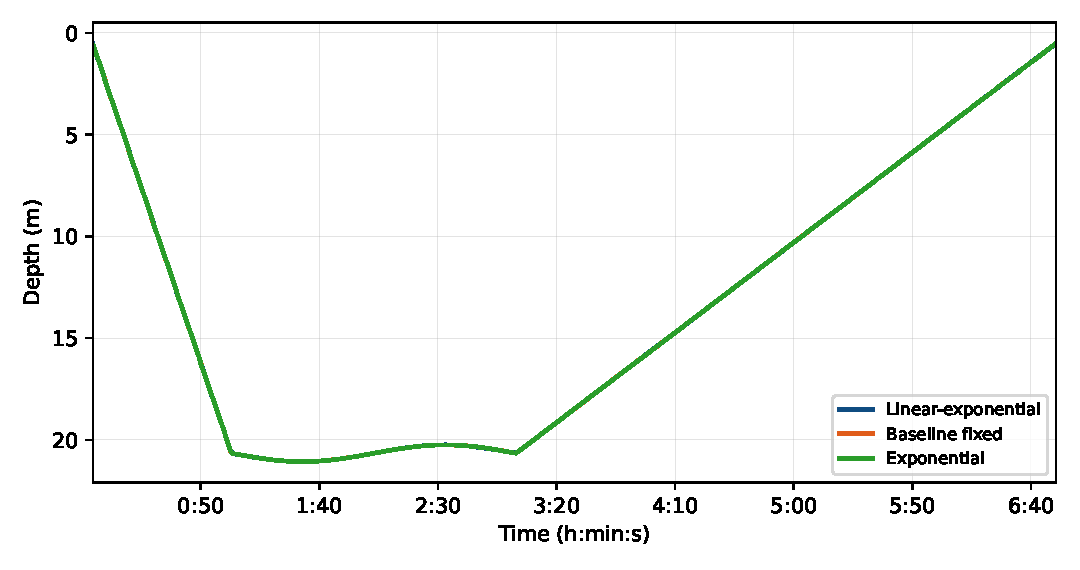
\includegraphics[width=0.9\textwidth]{figures/results/profile_20m.pdf}
\caption{Simulated Depth of 20m profile}
\label{fig:profile_20m}
\end{figure}

\begin{figure}[htbp]
\centering
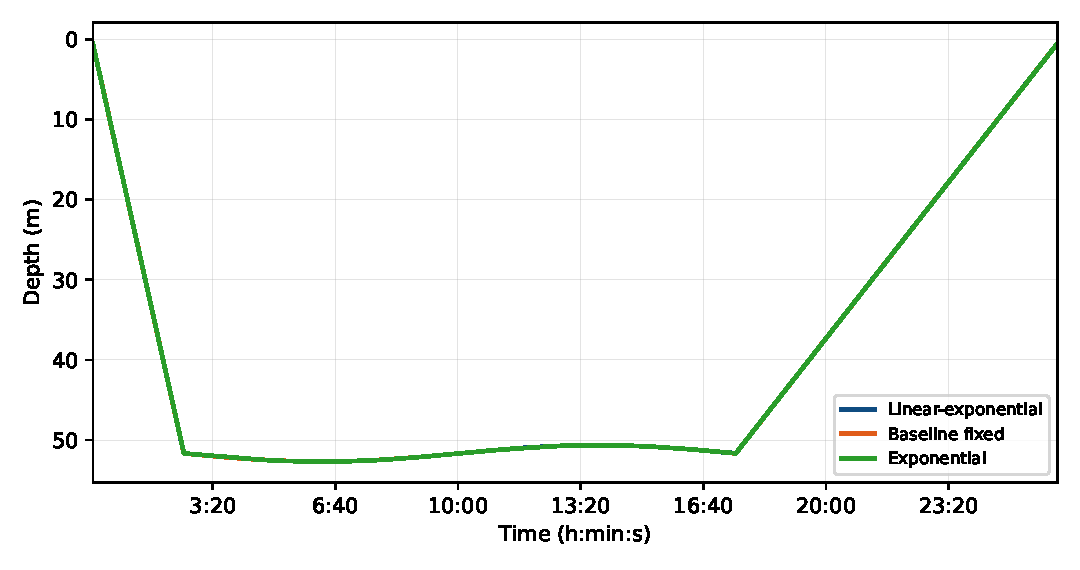
\includegraphics[width=0.9\textwidth]{figures/results/profile_50m.pdf}
\caption{Simulated Depth of 50m profile using the lin-exp decompression algorithm}
\label{fig:profile_50m}
\end{figure}

\begin{figure}[htbp]
\centering
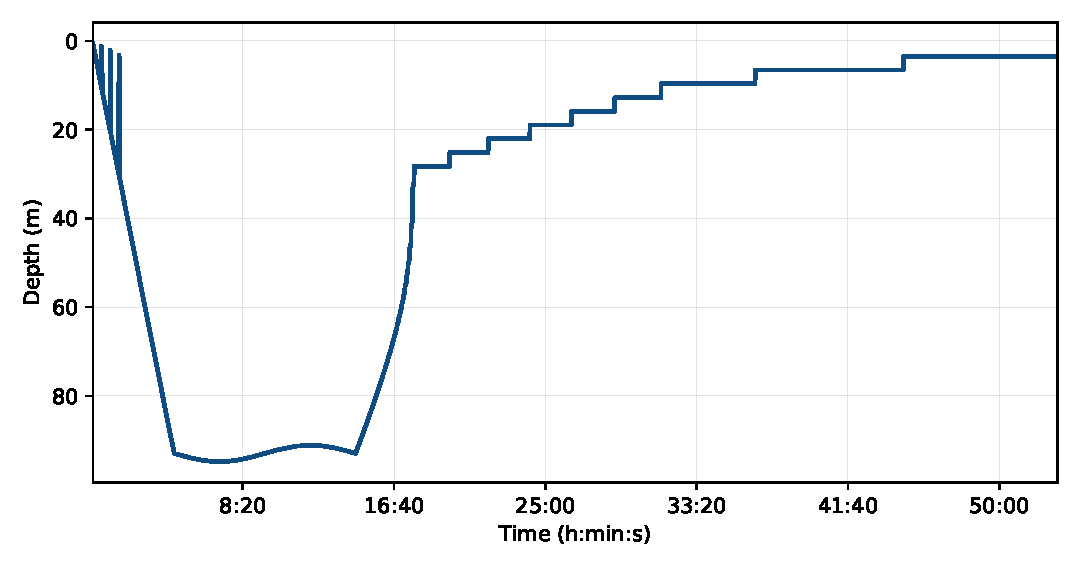
\includegraphics[width=0.9\textwidth]{figures/results/profile_90m.pdf}
\caption{Simulated Depth of 90m profile using the lin-exp decompression algorithm}
\label{fig:profile_90m}
\end{figure}

\section{\gls{o2tox} Algorithm results}
The implemented oxygen toxicity algorithm is only differential, runs on just one new measurement, and thus is comparatively cheap. 
The cycle count per execution of the fixed-rate algorithm, $235 \pm 2$, is only $10\%$ smaller than the execution of \gls{o2tox} itself, which is $266 \pm 2$.
This difference will become larger if more samples are used per-iteration.
The variable rate algorithms are on average $12.16\times$ more expensive, $1858 \pm 32$.

\begin{table}[htbp]
\centering
\small
\renewcommand{\arraystretch}{1.15}
\resizebox{\textwidth}{!}{%
\begin{tabular}{llrrrrrrrrrr}
\toprule
Configuration & Profile & Samples & Avg cycles & Avg [\si{\micro\second}] & Median cycles & Median [\si{\micro\second}] & Min cycles & Min [\si{\micro\second}] & Max cycles & Max [\si{\micro\second}] & Total cycles & Total [\si{\milli\second}] \\
\midrule
Baseline fixed & 20m & 8 & 265 & 16.6 & 265 & 16.6 & 265 & 16.6 & 265 & 16.6 & 2120 & 0.1 \\
Baseline fixed & 50m & 42 & 266 & 16.6 & 266 & 16.6 & 266 & 16.6 & 266 & 16.6 & 11172 & 0.7 \\
Baseline fixed & 90m & 87 & 266 & 16.6 & 266 & 16.6 & 266 & 16.6 & 266 & 16.6 & 23142 & 1.4 \\
Exponential & 20m & 1 & 265 & 16.6 & 265 & 16.6 & 265 & 16.6 & 265 & 16.6 & 265 & 0.0 \\
Exponential & 50m & 27 & 265 & 16.6 & 265 & 16.6 & 265 & 16.6 & 265 & 16.6 & 7155 & 0.4 \\
Exponential & 90m & 26 & 266 & 16.6 & 266 & 16.6 & 266 & 16.6 & 266 & 16.6 & 6916 & 0.4 \\
Linear-exponential & 20m & 1 & 267 & 16.7 & 267 & 16.7 & 267 & 16.7 & 267 & 16.7 & 267 & 0.0 \\
Linear-exponential & 50m & 34 & 266 & 16.6 & 266 & 16.6 & 266 & 16.6 & 266 & 16.6 & 9044 & 0.6 \\
Linear-exponential & 90m & 27 & 265 & 16.6 & 265 & 16.6 & 265 & 16.6 & 265 & 16.6 & 7155 & 0.4 \\
\bottomrule
\end{tabular}%
}
\caption{O\textsubscript{2} toxicity computation time across profiles and configurations}
\label{tab:timing_o2tox}
\end{table}

\begin{table}[htbp]
\centering
\small
\renewcommand{\arraystretch}{1.15}
\resizebox{\textwidth}{!}{%
\begin{tabular}{llrrrrrrrrr}
\toprule
Configuration & Profile & Samples & Avg cycles & Avg [\si{\micro\second}] & Min cycles & Min [\si{\micro\second}] & Max cycles & Max [\si{\micro\second}] & Total cycles & Total [\si{\milli\second}] \\
\midrule
Baseline fixed & 20m & 1833 & 237 & 14.8 & 237 & 14.8 & 237 & 14.8 & 434421 & 27.2 \\
Baseline fixed & 50m & 7778 & 234 & 14.6 & 234 & 14.6 & 234 & 14.6 & 1820052 & 113.8 \\
Baseline fixed & 90m & 13626 & 235 & 14.7 & 235 & 14.7 & 235 & 14.7 & 3202110 & 200.1 \\
Exponential & 20m & 1649 & 1825 & 114.1 & 1124 & 70.2 & 1826 & 114.1 & 3010372 & 188.1 \\
Exponential & 50m & 8402 & 1888 & 118.0 & 1482 & 92.6 & 1955 & 122.2 & 15867697 & 991.7 \\
Exponential & 90m & 13279 & 1860 & 116.2 & 1120 & 70.0 & 1955 & 122.2 & 24706189 & 1544.1 \\
Linear-exponential & 20m & 1841 & 1826 & 114.1 & 1124 & 70.2 & 1842 & 115.1 & 3362310 & 210.1 \\
Linear-exponential & 50m & 8563 & 1890 & 118.1 & 1126 & 70.4 & 1955 & 122.2 & 16190905 & 1011.9 \\
Linear-exponential & 90m & 14035 & 1854 & 115.9 & 1116 & 69.8 & 1946 & 121.6 & 26025090 & 1626.6 \\
\bottomrule
\end{tabular}%
}
\caption{O\textsubscript{2} toxicity rate-algorithm execution time across profiles and configurations}
\label{tab:timing_o2tox_rate}
\end{table}


Compared to the fixed rate baseline, the \gls{o2tox} algorithm is executed $0.65\times$ and $0.82\times$ as often on the $\SI{50}{\meter}$ profile, $0.15\times$ and $0.25\times$ as often on the $\SI{90}{\meter}$ profile. For  the shallow dive to $\SI{20}{\meter}$, no execution is required following the variable rate algorithm.

\begin{table}[htbp]
\centering
\small
\renewcommand{\arraystretch}{1.15}
\resizebox{\textwidth}{!}{%
\begin{tabular}{llrrrrr}
\toprule
Config. & Depth & Dec. & Due & Not due & Avg skip. [s] & Max skip. [s] \\
\midrule
Baseline & 20m & 487 & 6 & 481 & 47.567 & 135.836 \\
Baseline & 50m & 2099 & 42 & 2057 & 6.468 & 24.191 \\
Baseline & 90m & 3955 & 84 & 3871 & 3.209 & 17.005 \\
Exp. & 20m & 515 & 0 & 515 & 0.000 & 0.000 \\
Exp. & 50m & 2205 & 28 & 2177 & 8.689 & 37.064 \\
Exp. & 90m & 3872 & 20 & 3852 & 13.682 & 45.469 \\
Lin.-Exp. & 20m & 511 & 0 & 511 & 0.000 & 0.000 \\
Lin.-Exp. & 50m & 2295 & 19 & 2276 & 14.733 & 54.736 \\
Lin.-Exp. & 90m & 3700 & 19 & 3681 & 13.959 & 57.967 \\
\bottomrule
\end{tabular}%
}
\caption{O2Tox decision summary across profiles and configurations}
\label{tab:o2tox_decision_summary}
\end{table}


\section{Exponential \& Linear-Exponential Decompression Algorithm results}
The decompression obligation algorithms are significantly more expensive than the \gls{o2tox}, especially on dives with increased decompression obligation. 

The difference between the exponential and linear-exponential is small for shallow dives, on deeper dives, the average and total cycle counts are larger for the linear-exponential algorithm, which is at least partially caused by the tendency to create more (thus deeper) stops, and with more depth changes during decompression, more executions are required.

The decompression rate algorithm takes $1842 \pm^{34}_{32}$ cycles, while execution of the decompression schedule algorithm varies widely with the dive profile and current state, between $101'521$ and $886'860$ cycles, with the average close to the lower range of the spectrum on no-deco dives and $338614$ to $395242$ cycles.
The average execution overhead of an additional rate calculation is between $\frac{1837}{395'242} = 0.0046 = 0.4\%$ and $\frac{1810}{101'521} = 0.018 = 1.8\%$.

\begin{table}[htbp]
\centering
\small
\renewcommand{\arraystretch}{1.15}
\resizebox{\textwidth}{!}{%
\begin{tabular}{llrrrrrrrr}
\toprule
Configuration & Profile & Samples & Avg cycles & Avg [\si{\micro\second}] & Min cycles & Min [\si{\micro\second}] & Max cycles & Max [\si{\micro\second}] \\
\midrule
Baseline fixed & 20m & 1858 & 218 & 13.6 & 218 & 13.6 & 218 & 13.6 \\
Baseline fixed & 50m & 7505 & 218 & 13.6 & 218 & 13.6 & 218 & 13.6 \\
Baseline fixed & 90m & 13604 & 219 & 13.7 & 219 & 13.7 & 219 & 13.7 \\
Exponential & 20m & 1857 & 1809 & 113.1 & 1232 & 77.0 & 1950 & 121.9 \\
Exponential & 50m & 8879 & 1875 & 117.2 & 1231 & 76.9 & 1950 & 121.9 \\
Exponential & 90m & 16091 & 1842 & 115.1 & 1226 & 76.6 & 1946 & 121.6 \\
Linear-exponential & 20m & 2036 & 1810 & 113.1 & 1794 & 112.1 & 1935 & 120.9 \\
Linear-exponential & 50m & 8698 & 1878 & 117.4 & 1413 & 88.3 & 1952 & 122.0 \\
Linear-exponential & 90m & 14296 & 1837 & 114.8 & 1222 & 76.4 & 1941 & 121.3 \\
\bottomrule
\end{tabular}%
}
\caption{Decompression rate-algorithm execution time across profiles and configurations}
\label{tab:timing_deco_rate}
\end{table}

\begin{table}[htbp]
\centering
\small
\renewcommand{\arraystretch}{1.15}
\resizebox{\textwidth}{!}{%
\begin{tabular}{llrrrrrrrrrr}
\toprule
Config. & Depth & N & \multicolumn{2}{c}{Avg} & \multicolumn{2}{c}{Med.} & \multicolumn{2}{c}{Min} & \multicolumn{2}{c}{Max} & \multicolumn{2}{c}{Tot.} \\
\cmidrule(lr){4-5}\cmidrule(lr){6-7}\cmidrule(lr){8-9}\cmidrule(lr){10-11}\cmidrule(lr){12-13}
 & & & c. & [\si{\milli\second}] & c. & [\si{\milli\second}] & c. & [\si{\milli\second}] & c. & [\si{\milli\second}] & c. & [\si{\milli\second}] \\
\midrule
Baseline & 20m & 36 & 101811 & 6.36 & 101811 & 6.36 & 101811 & 6.36 & 101811 & 6.36 & 3665196 & 229.1 \\
Baseline & 50m & 137 & 189820 & 11.86 & 136057 & 8.50 & 101069 & 6.32 & 347567 & 21.72 & 26005350 & 1625.3 \\
Baseline & 90m & 249 & 371455 & 23.22 & 263000 & 16.44 & 101167 & 6.32 & 882588 & 55.16 & 92492527 & 5780.8 \\
Exp. & 20m & 8 & 101457 & 6.34 & 101457 & 6.34 & 101457 & 6.34 & 101457 & 6.34 & 811656 & 50.7 \\
Exp. & 50m & 88 & 177434 & 11.09 & 134590 & 8.41 & 101713 & 6.36 & 349706 & 21.86 & 15614217 & 975.9 \\
Exp. & 90m & 92 & 343165 & 21.45 & 150278 & 9.39 & 101549 & 6.35 & 885697 & 55.36 & 31571200 & 1973.2 \\
Lin.-Exp. & 20m & 9 & 101360 & 6.33 & 101360 & 6.33 & 101360 & 6.33 & 101360 & 6.33 & 912240 & 57.0 \\
Lin.-Exp. & 50m & 76 & 177419 & 11.09 & 134329 & 8.40 & 101523 & 6.35 & 349066 & 21.82 & 13483846 & 842.7 \\
Lin.-Exp. & 90m & 85 & 328362 & 20.52 & 256207 & 16.01 & 101521 & 6.35 & 885463 & 55.34 & 27910819 & 1744.4 \\
\bottomrule
\end{tabular}%
}
\caption{Decompression schedule computation time across profiles and configurations}
\label{tab:timing_deco_schedule}
\end{table}


Compared to the baseline execution count, depending on the profile, the variable rate algorithm leads to a $ 1.17\times$ to $6\times$ decrease in the execution count, which is in an almost linear relationship to the total cycle count spent on the computation of the decompression schedule. 
In the $\SI{50}{\meter}$ profile, the algorithms perform the worst, while in shallow and deep dives, the decrease in cycles is significant.

\input{./content/generated/05_results_exponential_decision_summary}
\begin{table}[htbp]
\centering
\small
\renewcommand{\arraystretch}{1.15}
\resizebox{\textwidth}{!}{%
\begin{tabular}{llrrrrr}
\toprule
Configuration & Profile & Decisions & Due & Not due & Avg skipped [s] & Max skipped [s] \\
\midrule
Baseline fixed & 20m & 575 & 520 & 55 & 2.096 & 5.111 \\
Baseline fixed & 50m & 5114 & 2410 & 2704 & 2.002 & 5.139 \\
Baseline fixed & 90m & 9742 & 4316 & 5426 & 2.027 & 5.112 \\
Exponential & 20m & 150 & 98 & 52 & 10.905 & 29.988 \\
Exponential & 50m & 4962 & 1957 & 3005 & 2.832 & 32.465 \\
Exponential & 90m & 8258 & 2371 & 5887 & 4.392 & 30.194 \\
Linear-exponential & 20m & 144 & 88 & 56 & 10.983 & 30.196 \\
Linear-exponential & 50m & 4657 & 1805 & 2852 & 2.875 & 30.192 \\
Linear-exponential & 90m & 7786 & 2021 & 5765 & 4.477 & 30.192 \\
\bottomrule
\end{tabular}%
}
\caption{Linear-exponential decompression decision summary across profiles and configurations}
\label{tab:linear_exponential_decision_summary}
\end{table}


 \section{Display Refresh results}
 The display refresh is the most expensive algorithm, partially due to current implementation using SPI over a Parallel Interface for simplicity in hardware and software. 
 Most executions update the internal state and skip the transfer to the display because the values on the display are unchanged.
 
 These executions which skip the transfer use no more than a few thousand, while full runs use up to $3.5$ million cycles.
 The display rate calculation 
 
 \begin{table}[htbp]
\centering
\small
\renewcommand{\arraystretch}{1.15}
\resizebox{\textwidth}{!}{%
\begin{tabular}{llrrrrr}
\toprule
Configuration & Profile & Decisions & Due & Not due & Avg skipped [s] & Max skipped [s] \\
\midrule
Baseline fixed & 20m & 64 & 22 & 42 & 11.740 & 127.893 \\
Baseline fixed & 50m & 204 & 39 & 165 & 6.372 & 61.985 \\
Baseline fixed & 90m & 637 & 93 & 544 & 2.890 & 16.504 \\
Exponential & 20m & 47 & 26 & 21 & 5.952 & 127.815 \\
Exponential & 50m & 148 & 27 & 121 & 9.293 & 67.870 \\
Exponential & 90m & 328 & 41 & 287 & 6.561 & 94.687 \\
Linear-exponential & 20m & 51 & 24 & 27 & 6.399 & 97.566 \\
Linear-exponential & 50m & 251 & 66 & 185 & 3.959 & 92.616 \\
Linear-exponential & 90m & 125 & 28 & 97 & 9.696 & 88.235 \\
\bottomrule
\end{tabular}%
}
\caption{Display refresh decision summary across profiles and configurations}
\label{tab:display_refresh_decision_summary}
\end{table}

 \begin{table}[htbp]
\centering
\small
\renewcommand{\arraystretch}{1.15}
\resizebox{\textwidth}{!}{%
\begin{tabular}{llrrrrrrrrrr}
\toprule
Configuration & Profile & Samples & Avg cycles & Avg [\si{\milli\second}] & Median cycles & Median [\si{\milli\second}] & Min cycles & Min [\si{\milli\second}] & Max cycles & Max [\si{\milli\second}] & Total cycles & Total [\si{\second}] \\
\midrule
Baseline fixed & 20m & 87 & 122403 & 7.65 & 10293 & 0.64 & 233 & 0.01 & 3244774 & 202.80 & 10649112 & 0.666 \\
Baseline fixed & 50m & 230 & 164918 & 10.31 & 21703 & 1.36 & 203 & 0.01 & 1928751 & 120.55 & 37931332 & 2.371 \\
Baseline fixed & 90m & 703 & 513642 & 32.10 & 21531 & 1.35 & 2115 & 0.13 & 3022821 & 188.93 & 361090882 & 22.568 \\
Exponential & 20m & 64 & 11752 & 0.73 & 10278 & 0.64 & 27 & 0.00 & 324734 & 20.30 & 752142 & 0.047 \\
Exponential & 50m & 151 & 211678 & 13.23 & 21760 & 1.36 & 2176 & 0.14 & 1919301 & 119.96 & 31963506 & 1.998 \\
Exponential & 90m & 374 & 525135 & 32.82 & 21204 & 1.33 & 2114 & 0.13 & 3040295 & 190.02 & 196400848 & 12.275 \\
Linear-exponential & 20m & 60 & 115936 & 7.25 & 10273 & 0.64 & 1023 & 0.06 & 3239318 & 202.46 & 6956178 & 0.435 \\
Linear-exponential & 50m & 261 & 141362 & 8.84 & 10673 & 0.67 & 1026 & 0.06 & 3242194 & 202.64 & 36895495 & 2.306 \\
Linear-exponential & 90m & 184 & 177304 & 11.08 & 21183 & 1.32 & 246 & 0.02 & 3022192 & 188.89 & 32624104 & 2.039 \\
\bottomrule
\end{tabular}%
}
\caption{Display refresh execution time across profiles and configurations}
\label{tab:timing_display_refresh}
\end{table}


% Based on Template from IIS, ETHz
%%%%%%%%%%%%%%%%%%%%%%%%%%%%%%%%%%%%%%%%%%%%%%%%%%%%%%%%%%%%%%%%%%%%%%%
%%%%%%%%%%%%%%%%%%%%%%%%%%%%%%%%%%%%%%%%%%%%%%%%%%%%%%%%%%%%%%%%%%%%%%%
%%%%%                                                                 %
%%%%%     <file_name>.tex                                             %
%%%%%                                                                 %
%%%%% Author:      <author>                                           %
%%%%% Created:     <date>                                             %
%%%%% Description: <description>                                      %
%%%%%                                                                 %
%%%%%%%%%%%%%%%%%%%%%%%%%%%%%%%%%%%%%%%%%%%%%%%%%%%%%%%%%%%%%%%%%%%%%%%
%%%%%%%%%%%%%%%%%%%%%%%%%%%%%%%%%%%%%%%%%%%%%%%%%%%%%%%%%%%%%%%%%%%%%%%

\chapter{Discussion}
% Draw your conclusions from the results you achieved and summarize your
% contributions. Comparisons (e.g., of hardware figures) with related
% work are also appropriate here. Point out things that could or need to
% be investigated further.

The results presented in Section \ref{section:results} are reproducible on the used hardware with the given software and will be interpreted in the following subsection.

\section{Impact of variable rate algorithms}
From this data, the following conclusions can be drawn: 

\begin{itemize}
    \item With the introduction of variable-rate algorithms, the number of cycles spent on calculating decompression schedules can be reduced by a significant amount. After reviewing the differences in actual decompression schedules, no significant differences, more than a few seconds can be observed over the up to $\SI{80}{\minute}$-long decompression dives.
    \item For less expensive algorithms like the \gls{o2tox} algorithm, the cost of running a more complex scheduling algorithm outweighs the benefit gained by running the algorithm less often.
    \item The difference in cycle count between the linear and linear-exponential algorithm does not exceed 
\end{itemize}

\section{Limitations}
\begin{itemize}
    \item Algorithms not yet optimized for performance 
    \item Consumed energy dominated by display, LEDs in this case
    \item => no energy comparison measurement or calculation
    \item \gls{mcu} running around 2.3-2.5V due to missing resistor in I2C Level Shifter usage on \gls{pcb}
    \item Core Frequency impact not measured (though cycle count should be accurate, just variation in idle cycle count expected)
    \item No standard libraries, algorithm implementations, rate algorithms used
\end{itemize}

Although some divers started to experiment with hydrogen for dives below $\SI{200}{\m}$, as is done in saturation diving, the number of scuba divers employing hydrogen-based mixtures remains negligible, and the currently available scientific literature is too limited to justify including hydrogen in the scope of this thesis project.

% Based on Template from IIS, ETHz
%%%%%%%%%%%%%%%%%%%%%%%%%%%%%%%%%%%%%%%%%%%%%%%%%%%%%%%%%%%%%%%%%%%%%%%
%%%%%%%%%%%%%%%%%%%%%%%%%%%%%%%%%%%%%%%%%%%%%%%%%%%%%%%%%%%%%%%%%%%%%%%
%%%%%                                                                 %
%%%%%     <file_name>.tex                                             %
%%%%%                                                                 %
%%%%% Author:      <author>                                           %
%%%%% Created:     <date>                                             %
%%%%% Description: <description>                                      %
%%%%%                                                                 %
%%%%%%%%%%%%%%%%%%%%%%%%%%%%%%%%%%%%%%%%%%%%%%%%%%%%%%%%%%%%%%%%%%%%%%%
%%%%%%%%%%%%%%%%%%%%%%%%%%%%%%%%%%%%%%%%%%%%%%%%%%%%%%%%%%%%%%%%%%%%%%%

\chapter{Conclusion and Future Work}
Short chapter on the conclusions you can draw from your work, and what is still to be done (and what contributions the students after you could make).


%%%%%
%%%%% Start of additional parts.
%%%%%
\appendix

% Based on Template from IIS, ETHz
%%%%%%%%%%%%%%%%%%%%%%%%%%%%%%%%%%%%%%%%%%%%%%%%%%%%%%%%%%%%%%%%%%%%%%%
%%%%%%%%%%%%%%%%%%%%%%%%%%%%%%%%%%%%%%%%%%%%%%%%%%%%%%%%%%%%%%%%%%%%%%%
%%%%%                                                                 %
%%%%%     <file_name>.tex                                             %
%%%%%                                                                 %
%%%%% Author:      <author>                                           %
%%%%% Created:     <date>                                             %
%%%%% Description: <description>                                      %
%%%%%                                                                 %
%%%%%%%%%%%%%%%%%%%%%%%%%%%%%%%%%%%%%%%%%%%%%%%%%%%%%%%%%%%%%%%%%%%%%%%
%%%%%%%%%%%%%%%%%%%%%%%%%%%%%%%%%%%%%%%%%%%%%%%%%%%%%%%%%%%%%%%%%%%%%%%

\chapter{Task Description}
Include the task description \textbf{pdf} you got from your
assistant(s) with the \shell{\textbackslash includepdf} command.
% include the task description pdf!
%\includepdf[pages=-, turn=false, scale=0.9]{../../task/TaskDescription.pdf}


\chapter{Declaration of Originality}\label{chap:originality}
Include the declaration of authorship with the \shell{\textbackslash
  includepdf} command (sign it and scan it). For more information
about plagiarism, please visit
\url{https://www.ethz.ch/students/en/studies/performance-assessments/plagiarism.html}

\begin{itemize}
\item \textbf{English version:}
  \url{https://www.ethz.ch/content/dam/ethz/main/education/rechtliches-abschluesse/leistungskontrollen/declaration-originality.pdf}
\item \textbf{German version:}
  \url{https://www.ethz.ch/content/dam/ethz/main/education/rechtliches-abschluesse/leistungskontrollen/plagiat-eigenstaendigkeitserklaerung.pdf}
\end{itemize}

% include the signed declaration of authorship!
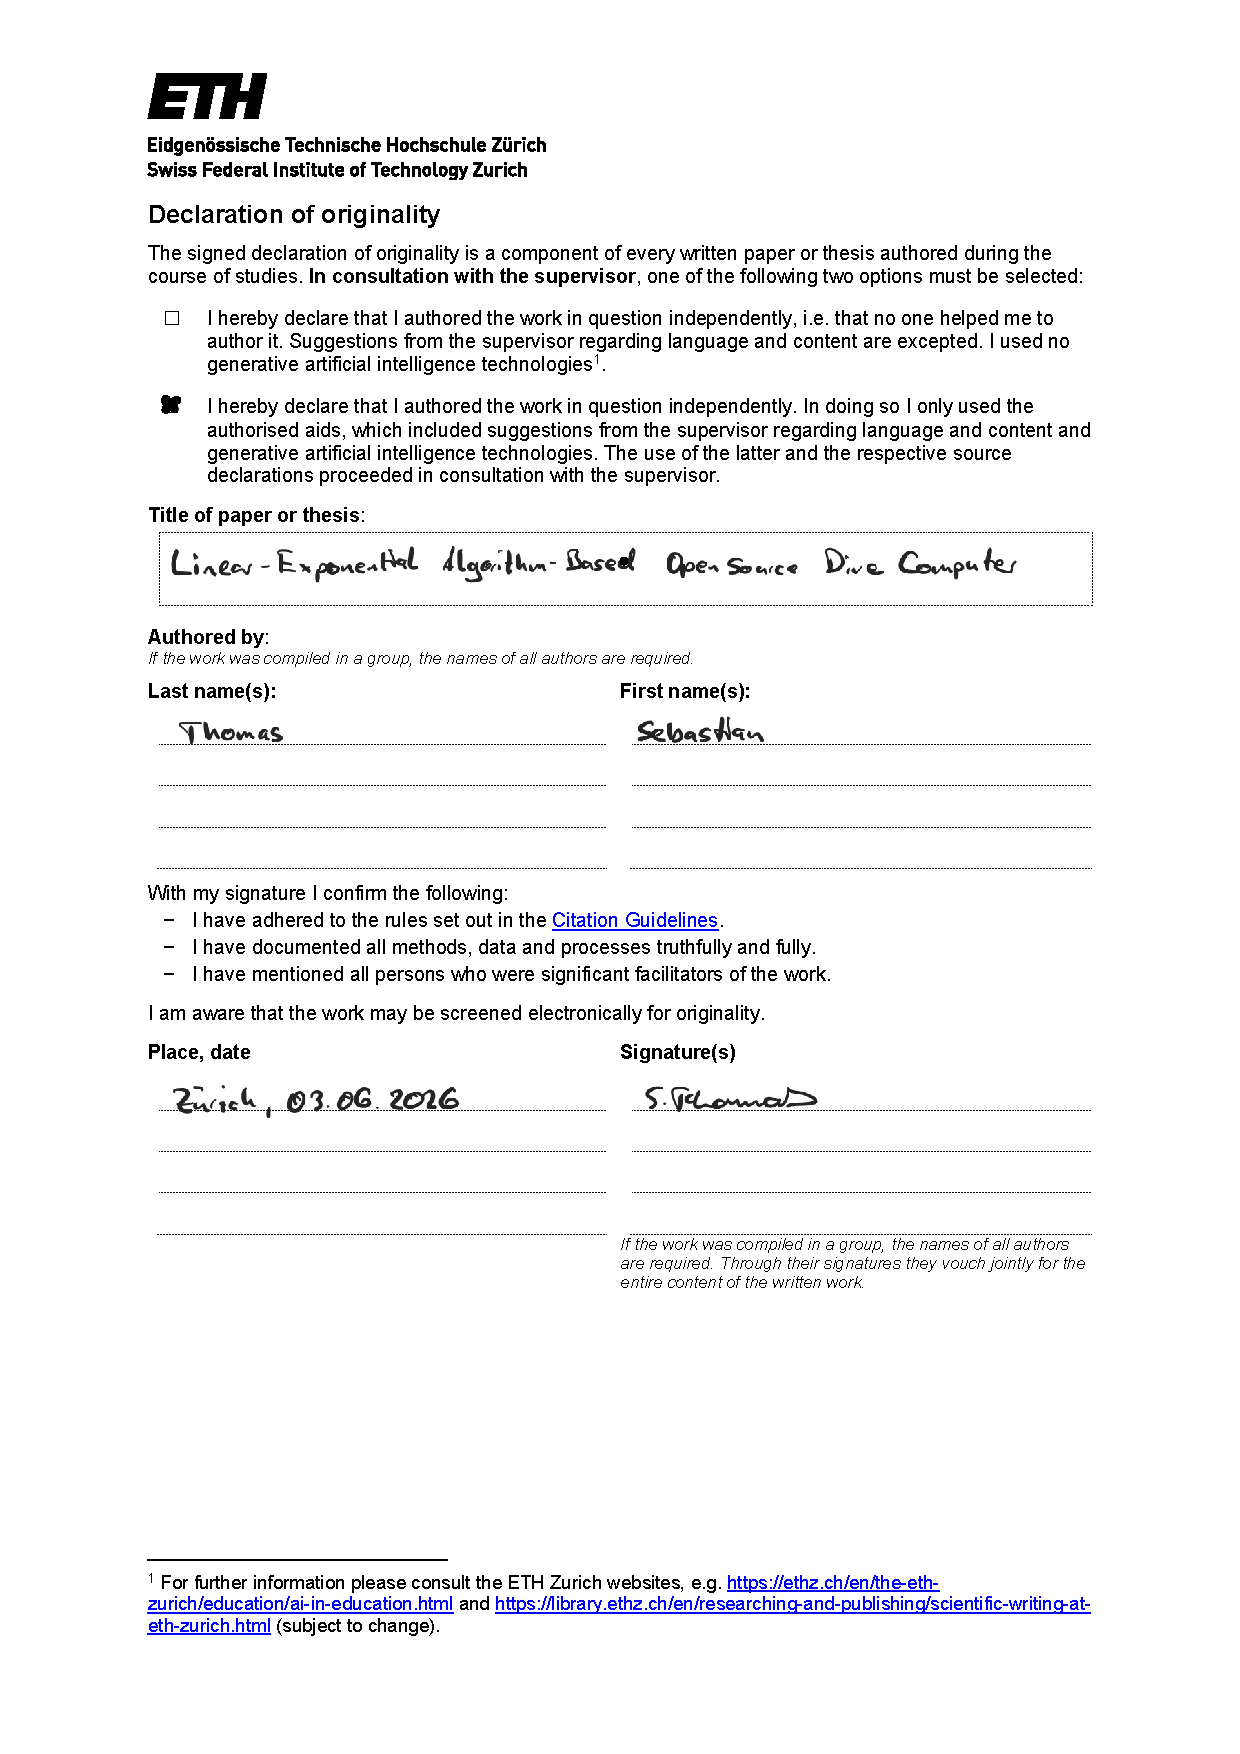
\includepdf[pages=-, turn=false, scale=0.9]{./figures/declaration_of_originality}


\chapter{(optional) File Structure}
Describe how the project directories/files are organized, e.g.:

\begin{flushleft}
\dirtree{%
.1 /.
  .2 README \DTcomment{A README with some general information about the project.}.
  .2 01\_report \DTcomment{The source files of the project report.}.
  .2 02\_presentation \DTcomment{The source files of the presentation.}.
  .2 03\_designflow \DTcomment{Some designflow-specific files.}.
}
\end{flushleft}

What needs to be done to run an RTL simulation (stimuli generation,
compilation...)?


\chapter{(optional) Datasets}
If you have a data set comprising several test images, you could
depict and describe them here. Use a simple naming scheme such that
you can easily refer to certain elements of this data set in the text.


\chapter{(optional) More Evaluation Results}
If you conducted an extensive evaluation you could move surplus
graphs/results to the appendix.

\backmatter

% Print the main glossary.
% optional Section
\printglossary[type=main,title=Glossary]


% Print the bibliography.
% \nocite*{} to be removed by the student
\nocite*{} % Print non-cited references as well.
\bibliographystyle{IEEEtran}
\bibliography{IEEEabrv,./bib/main}


\end{document}
%%%%%%%%%%%%%%%%%%%%%%%%%%%%%%%%%%%%%%%%%%%%%%%%%%%%%%%%%%%%%%%%%%%%%%%
%%%%%                                                                 %
%%%%%     End of Document                                             %
%%%%%                                                                 %
%%%%%%%%%%%%%%%%%%%%%%%%%%%%%%%%%%%%%%%%%%%%%%%%%%%%%%%%%%%%%%%%%%%%%%%
